\documentclass{article}
\usepackage{amsmath}
\usepackage[margin=3cm]{geometry}

\makeatletter 
\renewcommand{\fnum@figure}{Supplementary \figurename~\thefigure}
\renewcommand{\fnum@table}{Supplementary \tablename~\thetable}
\makeatother

\usepackage[labelfont=bf]{caption}
\usepackage{subcaption}
\usepackage{graphicx}
\newcommand{\beachmat}{\textit{beachmat}}
\newcommand{\code}[1]{\texttt{#1}}

\begin{document}

\begin{titlepage}
\vspace*{3cm}
\begin{center}


{\LARGE
beachmat: a Bioconductor C++ API for accessing single-cell genomics data from a variety of R matrix types
\par}

\vspace{0.75cm}

{\Large
    \textsc{Supplementary Materials}
\par
}
\vspace{0.75cm}

\large
by


\vspace{0.75cm}
Aaron T. L. Lun$^1$,
Herv\'e Pag\`es$^2$,
Mike L. Smith$^3$

\vspace{1cm}
\begin{minipage}{0.9\textwidth}
\begin{flushleft}
$^1$Cancer Research UK Cambridge Institute, University of Cambridge, Li Ka Shing Centre, Robinson Way, Cambridge CB2 0RE, United Kingdom \\[6pt]
$^2$Fred Hutchinson Cancer Research Center, 1100 Fairview Ave N, Seattle, WA 98109, USA \\[6pt]
$^3$European Molecular Biology Laboratory (EMBL), Genome Biology Unit, 69117 Heidelberg, Germany \\[6pt]
\end{flushleft}
\end{minipage}

\vspace{1.5cm}
{\large \today{}}

\vspace*{\fill}
\end{center}
\end{titlepage}

\providecommand{\myceil}[1]{\left \lceil #1 \right \rceil }

\section{Optimizing HDF5 chunk cache parameters}

\subsection{Overview}
Matrix data in HDF5 files can be partitioned into chunks \cite{hdf5chunk}, where each chunk is a submatrix of the same dimensions.
When a particular row or column of the matrix is requested, the HDF5 library will read all chunks that are overlapped by the requested row/column.
Each chunk is read from disk in its entirety, even if only a subset of the chunk is overlapped by the requested row/column.
This is wasteful as more data needs to be processed than is required for the current request.
To improve performance, chunks are cached in memory once they are read.
This means that they do not have to be re-read if a neighbouring row/column (overlapping the same set of chunks) is requested.
Chunks are then evicted from the cache once the memory limit is exceeded or if the hash indices overlap.
This behaviour allows efficient access to consecutive rows or columns in the HDF5 file.
However, some tuning of the parameters of the HDF5 chunk cache is required to achieve this, which we discuss below.

\subsection{Selecting the size of the chunk cache}
Assume that we have a chunk cache containing $S$ data values (this will have to be multiplied by the size of each value in bytes to obtain the actual cache size).
Denote the number of rows and columns of our matrix as $R$ and $C$, respectively. 
We further assume that these data are stored in a chunked layout, where the number of rows and columns in each chunk is $P$ and $Q$, respectively.

The chunk size $S$ should be chosen so that it can hold all chunks lying across a row or column.
Each chunk contains $PQ$ values, and each row and column overlaps $\myceil{C/Q}$ and $\myceil{R/P}$ chunks, respectively.
This reflects the fact that each chunk is stored in its entirety, even at the right/bottom edges of the matrix where each chunk may not be completely filled.
For row access, this means that 
\begin{equation}
S \ge \myceil{C/Q}PQ \;, 
\end{equation}
i.e., all chunks overlapping a particular row are held in memory. Simliarly, for column access, 
\begin{equation}
S \ge \myceil{R/P}PQ \;.
\end{equation}
This ensures that all chunks overlapping a particular row or column are retained in memory.
Otherwise, if the cache size is too small, existing chunks in the cache will be evicted before the current row or column is fully read.
(By default, the HDF5 chunk cache operates on a first-in-first-out basis when full.)
This would preclude the use of the cache to rapidly load data for the next row or column.

\subsection{Choosing the number of slots}
The chunk cache works by hashing the chunks according to their location in a one-dimensional array.
Consider a ``meta-matrix'' of chunks, where each chunk in the original matrix constitutes one entry in the meta-matrix.
A meta-row consists of all chunks along one row of this meta-matrix.
Similarly, a meta-column consists of all chunks along one column of the meta-matrix. 
Denote the number of meta-rows and meta-columns as $R_0$ and $C_0$, respectively.
Now, flatten the meta-matrix into a one-dimensional array of chunks, organized in row-major format.
The first chunk is assigned a hash index of 1 (technically 0, but we will use 1-based indexing for simplicity here).
The next chunk is assigned a hash index of 2, and so on.
When the hash index exceeds the number of cache slots $N$, it is reset to 1 for the next chunk.
This continues until a hash index is assigned to all entries of the meta-matrix.

The hash indices are important as two chunks with the same hash index cannot co-exist in the chunk cache.
This means that $N$ must be carefully chosen to ensure that all chunks in a meta-row or a meta-column have unique hash indices.
Otherwise, an existing chunk in the cache will be evicted by a newer chunk with the same hash index.
This would require the re-reading of the data in the older chunk when accessing the next row/column, defeating the purpose of the cache.
For a meta-row, guaranteeing unique indices is trivial as $N$ only needs to be chosen to be greater than or equal to $C_0$.

For a meta-column, more care is required.
Consider the first chunk lying in the first meta-column with a hash index of 1.
The hash index of 1 will only return to the first meta-column when the sequence $\{1, \ldots, N\}$ has been repeated enough times $m$ such that $mN$ is the smallest multiple of $C_0$.
Prior to this, all assigned values of the first meta-column will be unique.
This is obvious because non-unique values of the hash index in the first meta-column would imply an existing repeating structure, which is not possible without repeating the hash index of 1.
(The same logic can be applied to any other value of the hash index in any other meta-column.)
As the number of rows covered by $mN$ is equal to $mN/C_0$, we simply need to choose $N$ such that $mN/C_0 \ge R_0$.
This ensures that the hash index can never repeat itself for a given meta-column before hash indices are assigned to all entries in the meta-matrix.
The most direct approach is to set $N = kC_0 + 1$  where $k \in \mathbf{N}^+$ and $kC_0 +1 \ge R_0$.
This guarantees that the lowest common multiple of $N$ and $C_0$ is their product, and that $mN/C_0 \ge R_0$.

% Note that in the actual implementation, the meta rows are columns and vice versa.
% This is because rhdf5 internally transposes the data so that HDF5's row-major becomes R's column-major.

\subsection{Choosing the chunk dimensions}
The preceding text assumes that the chunk dimensions $P$ and $Q$ were set beforehand.
This is the case for existing HDF5 files, where the chunk layout must be specified during data set creation.
However, for new files, we have an opportunity to choose the chunk dimensions to optimize data access.

The number of disk reads involved in accessing each row is equal to the number of chunks across a row of the matrix, i.e., $\myceil{C/Q}$.
Once these are loaded into the cache, no more reads are required to access the next $P-1$ rows, i.e., data are held in memory for all $P$ rows simultaneously.
For comparison, consider a layout containing row chunks, i.e., each chunk is an entire row.
This provides the most efficient access to any single row as one read obtains all and only that row's data.
To access $P$ rows from a row-chunked layout, $P$ reads would be required.
Thus, for accessing consecutive rows with $P \times Q$ chunks, it is possible to perform as well as or better than the row-chunked layout if 
\begin{equation}
\myceil{C/Q} \le P \;.
\end{equation}
The same logic applies to column access, where $\myceil{R/P}$ reads are required to store data for $Q$ consecutive columns.
A layout with pure column chunks would require $Q$ reads to access the same data.
If 
\begin{equation}
\myceil{R/P} \le Q \;,
\end{equation}
we can also outperform the column-chunked layout for accessing data in consecutive columns.
Thus, by choosing $P$ and $Q$ to satisfy Inequalities~3 and 4, we can use a single file layout to achieve data access performance similar to or better than that of pure column- or row-based chunking.

Obviously, any arbitrarily large $P$ and $Q$ will satisfy Inequalities~3 and 4.
To avoid this, we use Inequalities~1 and 2 to determine the minimum chunk cache size.
The aim is to satisfy all of the inequalities while minimizing $S$ to reduce the memory overhead.
In general, this requires some numerical analysis to account for the discrete nature of the dimensions.
We obtain some approximate values by treating all variables as continuous, which allows us to satisfy all inequalities when $S \ge \max\{R\sqrt{C}, C\sqrt{R}\}$.
Once the smallest $S$ is obtained, the largest $P$ and $Q$ are easily determined.

%%% OVERVIEW:
% 3 and 4 require that PQ >= C and PQ >= R
% 1 and 2 require that S >= CP and S >= RQ

% Assume R >= C and RQ >= CP. 
% This means that we need PQ >= R and S >= RQ.
% The smallest value of S occurs at the smallest value of Q (as R is constant).
% The smallest value of Q is either CP/R or R/P. 
% If R/P >= CP/R, we get P <= R/C^0.5, which means that Q >= C^0.5.
% If R/P <= CP/R, we get P >= R/C^0.5, which means that Q >= C^0.5.
% Either way, this means that the smallest value of S is RC^0.5.

% Now assume that R <= C and RQ >= CP.
% This means that we need PQ >= C and S >= RQ.
% The smallest value of Q is now either C/P or CP/R.
% If C/P >= CP/R, we get P <= R^0.5, which means that Q >= C/R^0.5
% If C/P <= CP/R, we get P >= R^0.5, which means that Q >= C/R^0.5.
% Either way, this means that the smallest value of S is CR^0.5.
%
% By symmetry, we would get these two options if we swapped R <=> C and P <=> Q.

\subsection{Worked example of choosing chunk settings}
Say that we have a matrix $X$ with 20000 rows and 50000 columns.
Our approach suggests that we should choose $S$ as being greater than $50000\sqrt{20000} \approx 7071068$ for optimal access.
We set $S=8000000$ to simplify the later divisions, which corresponds to an in-memory size of 64 MB for double-precision values.
Our chunk dimensions are $P = S/50000 = 160$ and $Q = S/20000 = 400$.
In practice, one may wish to cap the cache size at the cost of some performance, lest too much memory be requested.

\textit{beachmat} provides functions to perform the above calculations given $R$ and $C$.
However, \textit{beachmat} will not automatically use the computed $P$ and $Q$ as the chunk dimensions for output \texttt{HDF5Matrix}.
This is because the optimal chunk dimensions depend on the anticipated access patterns, which are unknown to the \textit{beachmat} API at the time of file creation.
The choice of $P$ and $Q$ above is only optimized for consecutive row and column accesses, while the actual access pattern might be random (see Section~\ref{sec:random}).
Thus, the chunk dimensions must be manually chosen by the user/developer.
Obviously, this is irrelevant when accessing data from existing HDF5 files where the layout is already fixed.

\section{Performance of different HDF5 file layouts}

\subsection{Testing with simulated data}
We demonstrate the effect of the choice of file layout on access to HDF5-backed data.
For column access, we consider the performance of \beachmat{} with a contiguous layout, column-wise chunks with compression, and row-wise chunks.
The contiguous layout is the fastest as only one disk read needs to be performed per column (Supplementary Figure~\ref{fig:hdf5layout}).
Column-wise chunking also involves a single disk read per column, but is slower due to the overhead of decompression and chunk caching.
Rectangular chunking is slightly slower than column-wise chunks, despite the optimized size of the cache -- this is attributable to the time spent collecting data across multiple cached chunks.
As expected, row-wise chunks is the slowest as each column access effectively processes data from the entire matrix.

The results are reversed for row access, where row-wise chunking is the layout that provides the best performance with \beachmat{} (Supplementary Figure~\ref{fig:hdf5layout}).
This is expected as only one disk read is required per row, compared to multiple reads with column-wise chunking.
We emphasize that rectangular chunking is only slightly slower than row-wise chunking when the chunk cache is optimized.
This highlights the utility of rectangular chunks for both row and column accesses, compared to the other schemes where performance deteriorates rapidly for non-ideal access patterns.
The contiguous layout is also slow as multiple reads are required to access the non-contiguous data from each row.

\subsection{Dealing with random access}
\label{sec:random}

It should be stressed that these timings were generated with consecutive row and column accesses.
The chunk cache is not effective for a random access pattern, as there is no guarantee that the cached data will contain the next requested row or column.
(We omit the situation where the entire matrix is loaded into the cache.
If this were possible, a simple matrix representation would have sufficed.)
In such cases, pure row- or column-based chunks may be necessary for optimal performance.
However, the best layout is not clear at the time of file creation, especially for scRNA-seq data where it is sensible to access data by gene (row) or cell (column).
Switching from one layout to the other may be necessary throughout the course of an analysis that performs random queries on both rows and columns.

The \beachmat{} strategy implements a simple approach to converting an existing HDF5 file to a layout using row- or column-based chunks.
Consider an existing file with chunk dimensions of $(P_1, Q_1)$. 
Assume that we want to obtain a new file with chunk dimensions of $(1, Q_2)$, i.e., row-wise chunks containing $Q_2$ values.
We extract a submatrix of size $(P_1, Q_2)$ from the existing file and write it to the new file with the row-chunked layout.
This is repeated with the next submatrix of the same size along the next $Q_2$ columns, and the process is iterated until all columns have been read and written for these $P_1$ rows.
The size of the chunk cache is set to hold the single chunk that has not been completely read/written between iterations when $Q_2$ is not a multiple of $Q_1$.
We repeat this procedure with the next $P_1$ rows until the entire file has been processed.
To convert to column-based chunks of size $(P_2, 1)$, a submatrix of size $(P_2, Q_1)$ is extracted and written to file; this is repeated for the next $P_2$ rows, until all rows have been processed for these $Q_1$ columns; and the process is repeated with the next $Q_1$ columns until the entire file is rewritten.
The idea is to load read and write entire chunks as much as possible, reducing the number of redundant disk accesses.
Only a submatrix of the data needs to be held in memory at each iteration, which reduces the overhead of the conversion.

Converting from one layout to the other with the above strategy is fast, requiring only a few seconds for small matrices (Supplementary Figure~\ref{fig:hdf5rechunk}).
The time scales linearly with matrix size, so for a large data set with a million cells, it would take 2-3 hours.
This is minor compared to the time spent by the entire analysis.
Nonetheless, to maximize efficiency, all functions requiring column-based access (e.g., cell quality control and normalization) should be grouped together and executed first; 
this should be followed by a layout conversion step, and then by execution of functions requiring row-based access (e.g., gene-based processing).
An alternative option would be to store scRNA-seq data in both row- and column-chunked form (i.e., as two separate HDF5 data sets) to allow for both access patterns.
While this has some uses, it is difficult to ensure that both versions are synchronised throughout an interactive analysis.
Transformations applied to one data set must be applied to the other, which introduces considerable overhead as operations and disk accesses must be performed twice.

\small
\bibliography{ref}
\bibliographystyle{unsrt}

\newpage

\begin{figure}[bt]
    \centering
    \begin{subfigure}[b]{0.49\textwidth}
        \includegraphics[width=\textwidth]{../simulations/timings/pics/base_col.pdf}
        \caption{}
    \end{subfigure}
    \begin{subfigure}[b]{0.49\textwidth}
        \includegraphics[width=\textwidth]{../simulations/timings/pics/base_row.pdf}
        \caption{}
    \end{subfigure}
    \caption{Time required for column or row access of simple matrices using the \beachmat{} or \textit{Rcpp} APIs.
        (a) Column access time with respect to the number of columns, for a matrix with 10000 rows.
        (b) Row access time with respect to the number of rows, for a matrix with 1000 columns.
%        Access was timed after computing the column/row sums to ensure iteration with each API.
%        Each time represents the average of 10 simulations.
%        Standard errors were negligible and are not shown.
        Intervals between the horizontal dotted lines represent 2-fold increases in time.
    }
    \label{fig:basetime}
\end{figure}

\begin{figure}[bt]
    \centering
    \includegraphics[width=0.8\textwidth]{pics/sparse.pdf}
    \caption{A schematic of the column-sparse compressed matrix format, as implemented by the \texttt{dgCMatrix} class in the \textit{Matrix} package.
        The grey box represents a sparse matrix with zero entries indicated by the dots.
        The \texttt{x} vector stores all non-zero values, ordered in column-major format.
        The index of each element in \texttt{x} is shown in red.
        The \texttt{i} vector stores the row indices (blue) corresponding to the ordered non-zero values.
        The \texttt{p} vector stores the element index of the first non-zero value in each column (brown).
        The last element of \texttt{p} is always the total number of non-zero entries.
    }
    \label{fig:sparsefig}
\end{figure}

\begin{figure}[bt]
    \centering
    \begin{subfigure}[b]{0.49\textwidth}
        \includegraphics[width=\textwidth]{../simulations/timings/pics/sparse_col_density.pdf}
        \caption{}
    \end{subfigure}
    \begin{subfigure}[b]{0.49\textwidth}
        \includegraphics[width=\textwidth]{../simulations/timings/pics/sparse_col_ncol.pdf}
        \caption{}
    \end{subfigure}
    \caption{Column access times for CSC matrices using \beachmat{} (sparse) or \textit{RcppArmadillo}, compared to an equivalent simple matrix with \beachmat{} (simple).
        (a) Access times with respect to the density of non-zero entries as a percentage of all entries, for a matrix with 10000 rows and 1000 columns.
        (b) Access times with respect to the number of columns, for a matrix with 10000 rows and 1\% density.
        Horizontal dotted lines represent 2-fold increases in time.
    }
    \label{fig:sparsecol}
\end{figure}

\begin{figure}[bt]
    \begin{subfigure}[b]{0.49\textwidth}
        \includegraphics[width=\textwidth]{../simulations/timings/pics/HDF5_col_layout.pdf}
        \caption{}
    \end{subfigure}
    \begin{subfigure}[b]{0.49\textwidth}
        \includegraphics[width=\textwidth]{../simulations/timings/pics/HDF5_row_layout.pdf}
        \caption{}
    \end{subfigure}
    \caption{Column/row access times of \beachmat{} for \code{HDF5Matrix} objects constructed with different HDF5 file layouts, 
        i.e., contiguous, row- or column-chunking, or $40\times40$ rectangular chunks.
        (a) Column access times with respect to the number of columns, for a dense matrix with 1000 rows.
        (b) Row access times with respect to the number of rows, for a dense matrix with 100 columns.
        Horizontal dotted lines represent 2-fold increases in time.
    }
    \label{fig:hdf5layout}
\end{figure}

\begin{figure}[bt]
    \begin{subfigure}[bt]{0.49\textwidth}
        \includegraphics[width=\textwidth]{../simulations/timings/pics/HDF5_col_rechunk.pdf}
        \caption{}
    \end{subfigure}
    \begin{subfigure}[bt]{0.49\textwidth}
        \includegraphics[width=\textwidth]{../simulations/timings/pics/HDF5_row_rechunk.pdf}
        \caption{}
    \end{subfigure}
    \caption{Time required to convert from a column-based chunk layout to a row-based chunk layout, or vice versa.
        Each chunk contained 5000 values along a single row or column (or set to the corresponding dimension of the matrix, if it was smaller than 5000).
        Conversion times were recorded with respect to increasing number of (a) columns and (b) rows.
        All values represent the mean of 10 simulation iterations.
        Horizontal dotted lines represent 2-fold increases in time.
    }
    \label{fig:hdf5rechunk}
\end{figure}

\begin{figure}[bt]
    \begin{center}
        \includegraphics[width=\textwidth]{pics/rumours.png}
    \end{center}
    \caption{A screenshot of the 10X webpage where the 1 million neuron data set can be downloaded (see Methods for the URL).
    The relevant statement is highlighted in yellow.}
\end{figure}

\end{document}
